\section{Data Analysis}
\subsection{Analyzing Window Size}

Larger window sizes - (128, 96) and (128, 64) - performed best on INRIA (\ref{fig:window_size_inria}) and Caltech (\ref{fig:window_size_caltech}) datasets by capturing more contextual information, closely aligning with Dalal and Triggs' observations \cite{dalal_2005_histograms}. In contrast, PnPLO dataset showed better results with smaller windows - (112, 48) and (100, 50) - likely because they focus more on local features, reduce the amount of potentially confusing information, and avoid overfitting to the artificial characteristics of mannequins and statues (like display platforms)

\subsection{Analyzing Derivative Masks}

The holistic derivative mask (HDM) enhanced performance across all datasets, with particularly strong improvements on Caltech (\ref{fig:hdm_caltech}) and PnPLO (\ref{fig:hdm_pnplo}). The HDM approach preserves gradient information at object boundaries, crucial for detecting pedestrians in low-resolution images like those in the Caltech dataset \cite{dollar_2009_pedestrian}. While less pronounced on INRIA due to well-centered subjects with (generally) ample of surrounding margin \cite{dalal_2005_histograms}, HDM configurations still showed statistically significant improvements ($p=6\cdot 10^{-9}$), as illustrated in figure \ref{fig:best_hdm_inria}.


\begin{figure}
    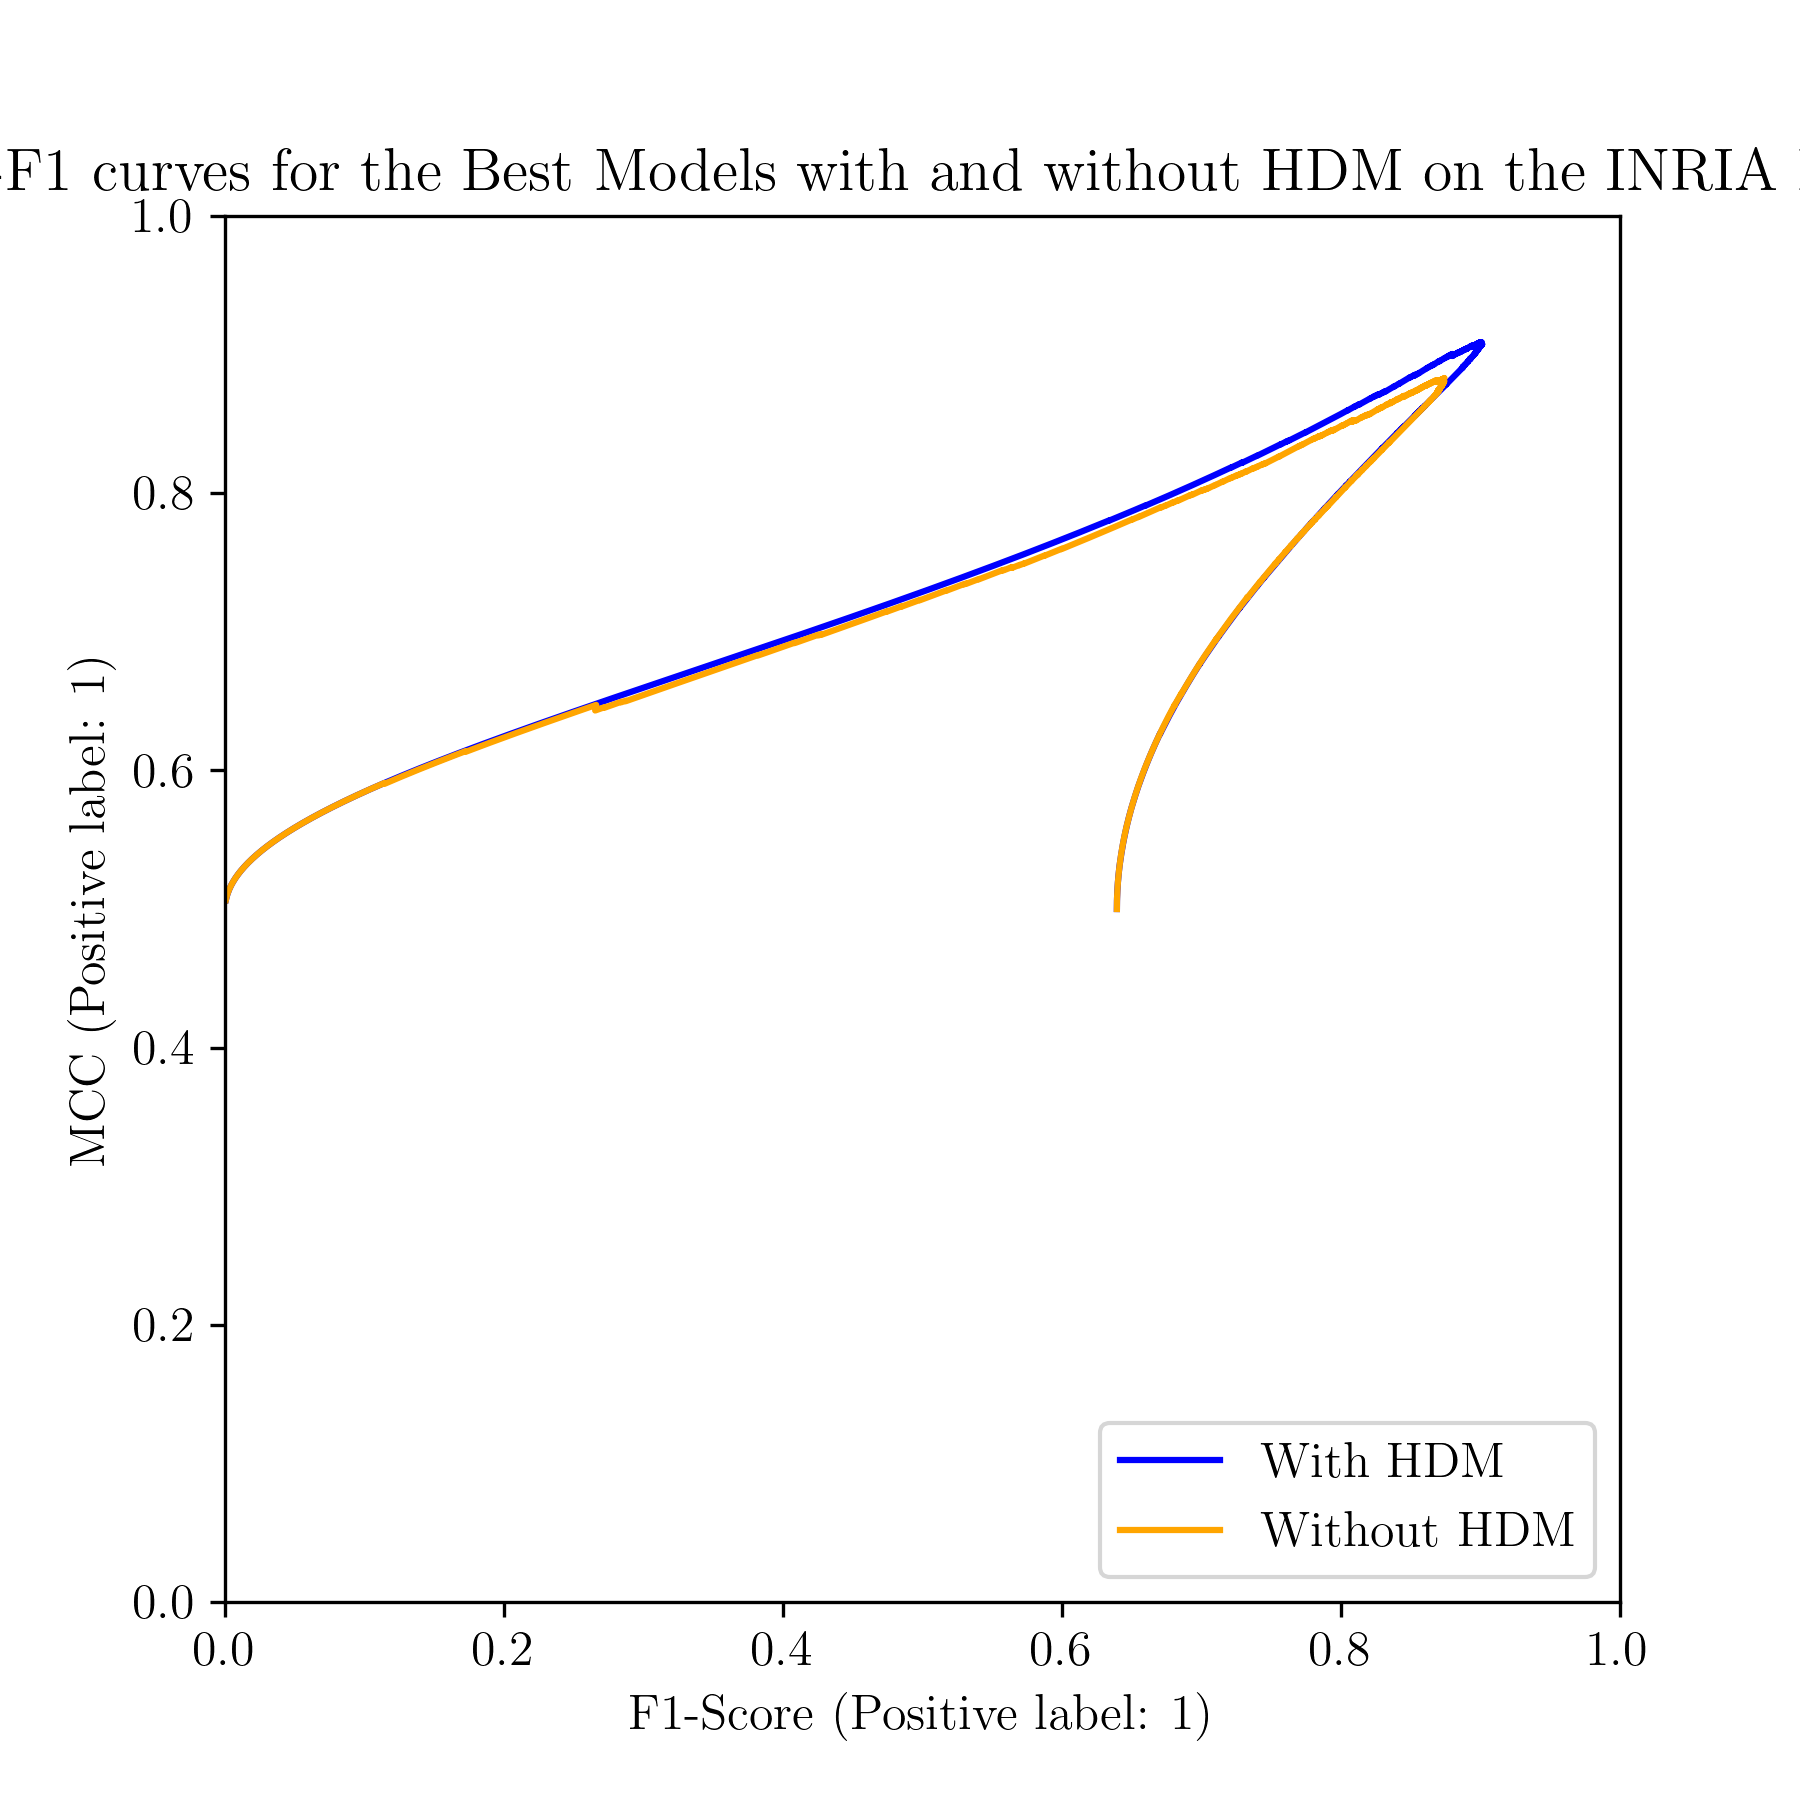
\includegraphics[width=0.6\linewidth]{best_hdm_mcc_f1_inria.png}
    \caption{
        The best performing configurations on the INRIA data set with and without the holistic derivative mask (HDM). 
    }
    \label{fig:best_hdm_inria}
\end{figure}


\subsection{Analyzing Orientation Bin Sizes}

Experimental results (\ref{fig:orientation_bins_inria}-\ref{fig:orientation_bins_total}) confirmed Dalal and Triggs' findings: increasing bin size beyond 9 yields minimal improvements \cite{dalal_2005_histograms} (all pairwise p-values $\sim 0.05$). This trend of diminishing returns can likely be attributed to the consistent edge orientations in human body shapes. Finer binning over the 0°-180° range (e.g., 13.8° intervals for 13 bins or 10° intervals for 18 bins) fails to capture significantly more discriminative information and only increases time of computation (as $\omega$ is a component of dimensionality in figure \ref{fig:correlation_with_best_fit}). Still, configurations with 18 bins show insignificantly higher MCC scores, meaning that the diminishing returns outpace the negative impact of increased dimensionality.

\subsection{Analyzing Block Density}

Heatmaps in figures \ref{fig:cell_block_heatmap_inria} through \ref{fig:cell_block_heatmap_total} show an optimal configuration comprised of (2,2) block size and (8,8) cell size for INRIA and PnPLO, with Caltech showing similar performance between (4,4) (4,4) and (2,2) (8,8) block density setups ($p=0.775$). Both density setups yield $16\times16$ pixel block areas, which appear to provide the optimal balance between local and global features (in contrast to the best performing $18\times18$ area in the seminal HOG paper \cite{dalal_2005_histograms}), as illustrated in figure \ref{fig:block_area}. Beyond this disagreement, other results are consistent with Dalal and Triggs' paper: smaller block sizes (e.g., (1,1)) fail to capture broader contextual information, while larger block sizes (e.g., (10,10)) lose focus on critical local features \cite{dalal_2005_histograms}.

\begin{figure}
    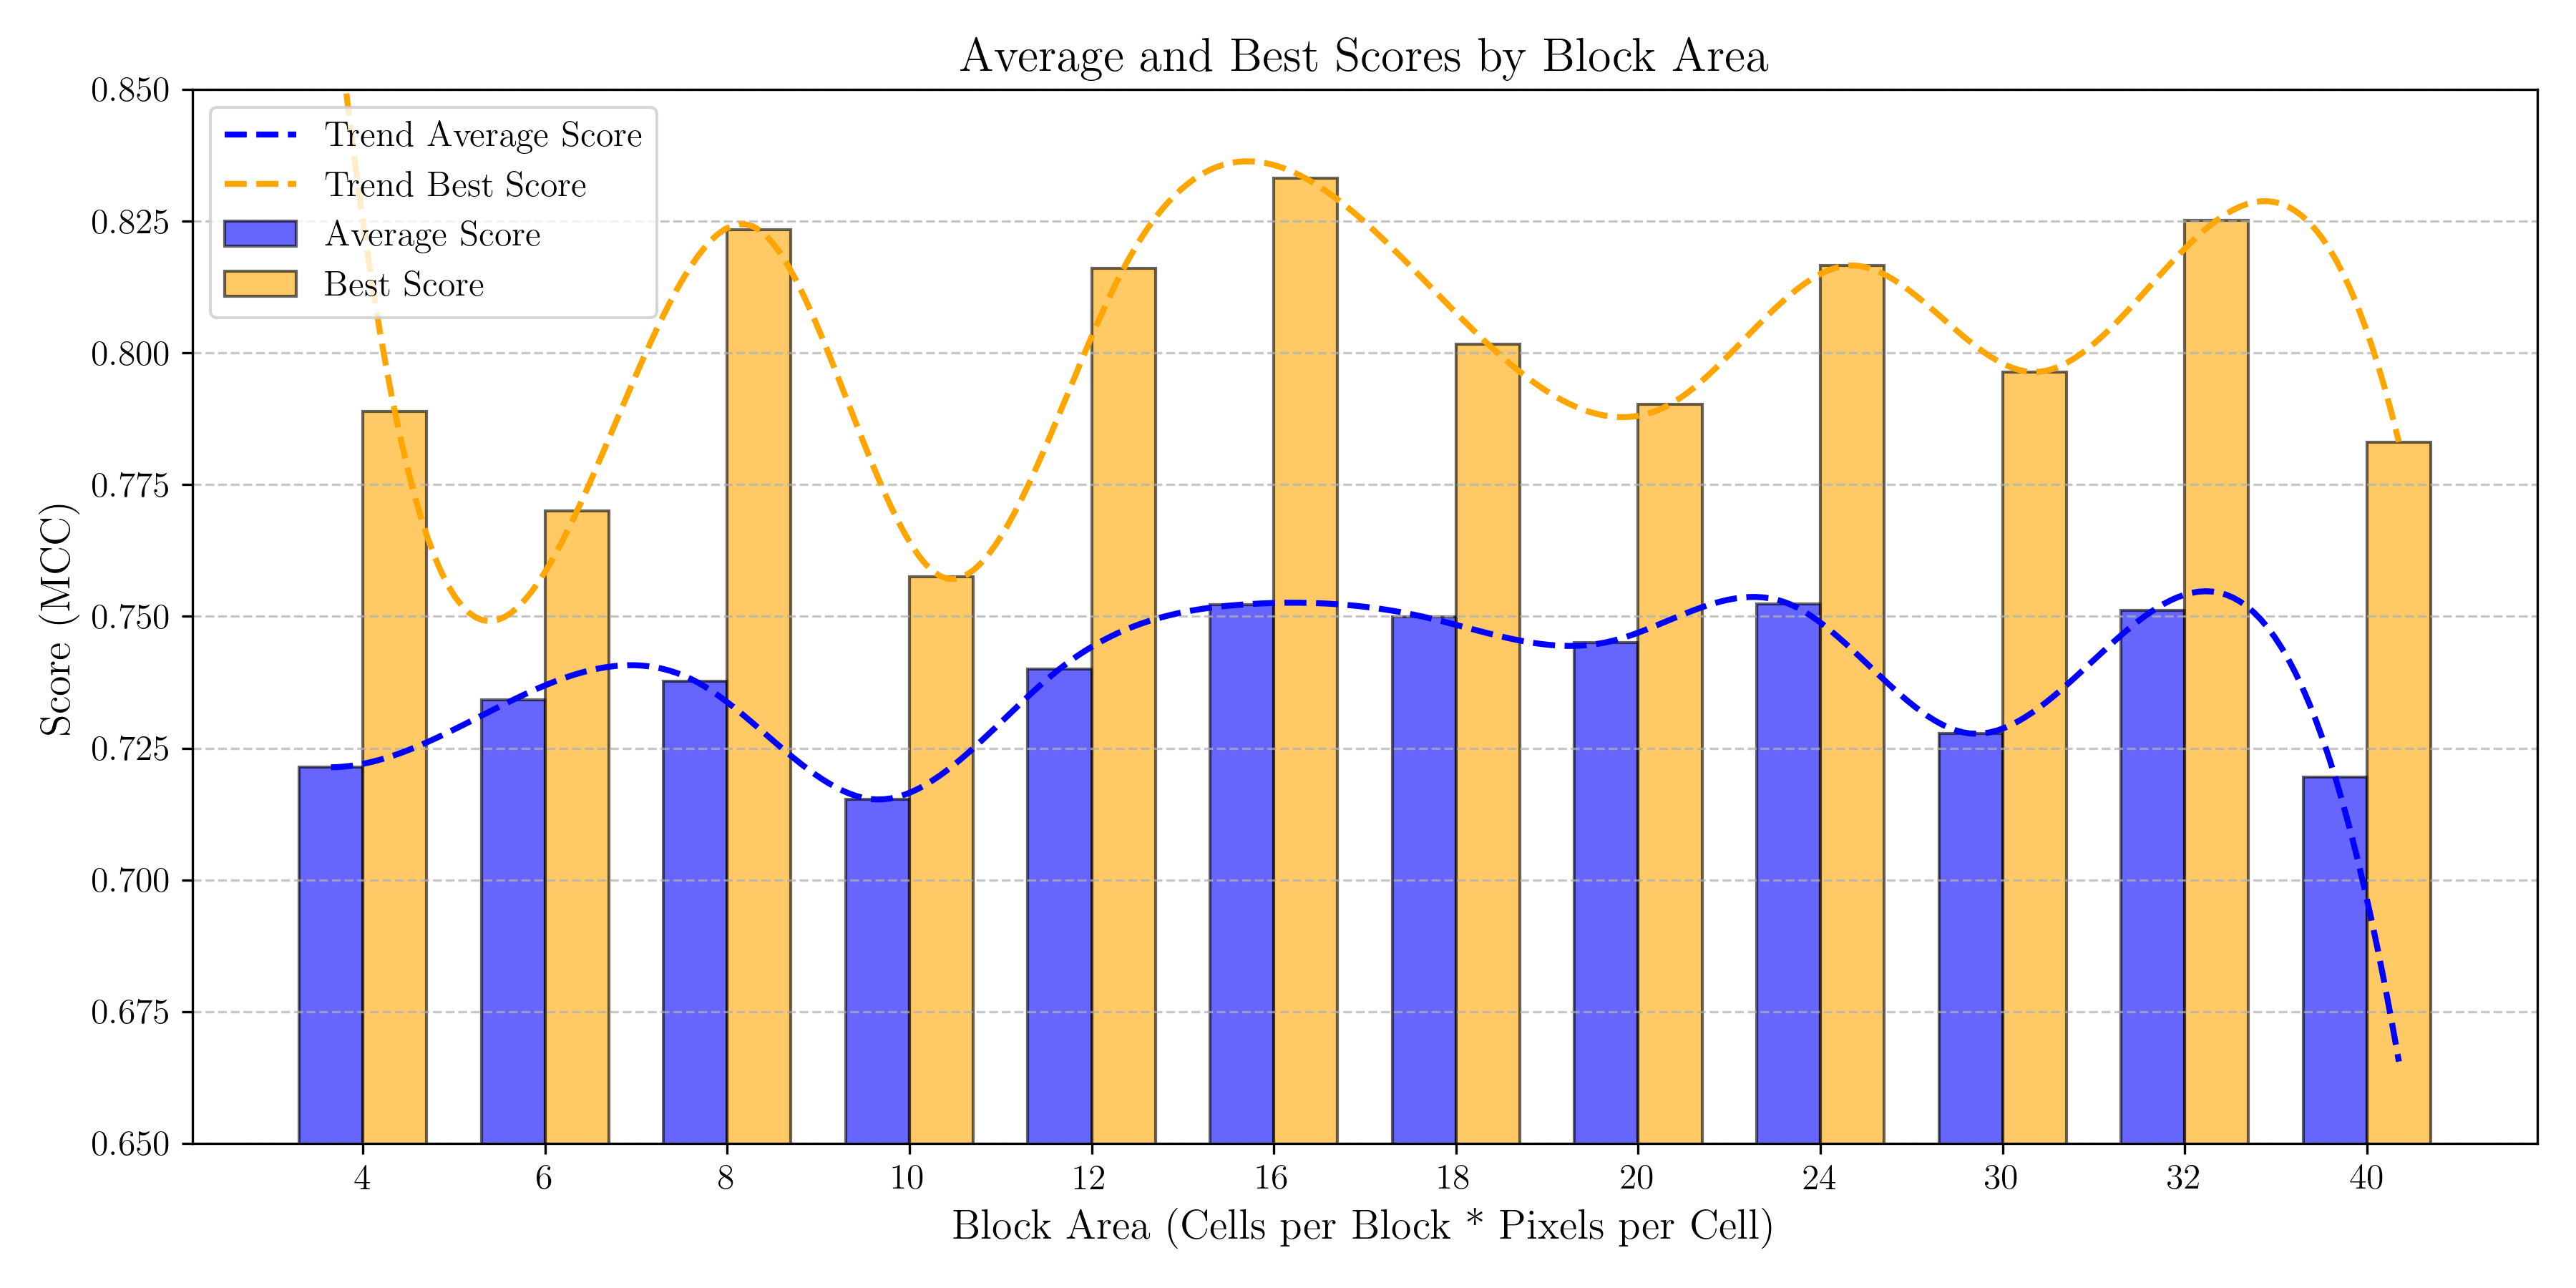
\includegraphics[width=\linewidth]{mcc_block_area.png}
    \caption{
        A bar chart of average and best MCC scores for each configuration's block area (defined as block width (or height) $\times$ cell width (or height)). 
    }
    \label{fig:block_area}
\end{figure}

\subsection{Analyzing Block Stride}

As in Dalal and Triggs' paper, higher stride values increases block overlap, which enhances detection performance, particularly for (4,4) blocks where 75\% overlap significantly outperformed 50\% overlap ($p=0.000534$). However, (2,2) blocks showed no significant difference between 50\% and 0\% overlap ($p=0.2911$), suggesting stride values of (2,2) could optimize computational efficiency for (2,2) blocks without compromising accuracy.